\chapter{Anomaly detection: Taxi calls}

\begin{description}
    \item[Anomaly] \marginnote{Anomaly}
        Event that deviates from the usual pattern.

    \item[Time series] \marginnote{Time series}
        Data with an ordering (e.g., chronological).
\end{description}



\section{Data}

The dataset is a time series and it is a \texttt{DataFrame} with the following fields:
\begin{descriptionlist}
    \item[\texttt{timestamp}] with a 30 minutes granularity.
    \item[\texttt{value}] number of calls.
\end{descriptionlist}

The label is a \texttt{Series} containing the timestamps of the anomalies.

An additional \texttt{DataFrame} contains information about the time window in which the anomalies happen:
\begin{descriptionlist}
    \item[\texttt{begin}] acceptable moment from which an anomaly can be detected.
    \item[\texttt{end}] acceptable moment from which there are no anomalies anymore.
\end{descriptionlist}

\begin{figure}[H]
    \centering
    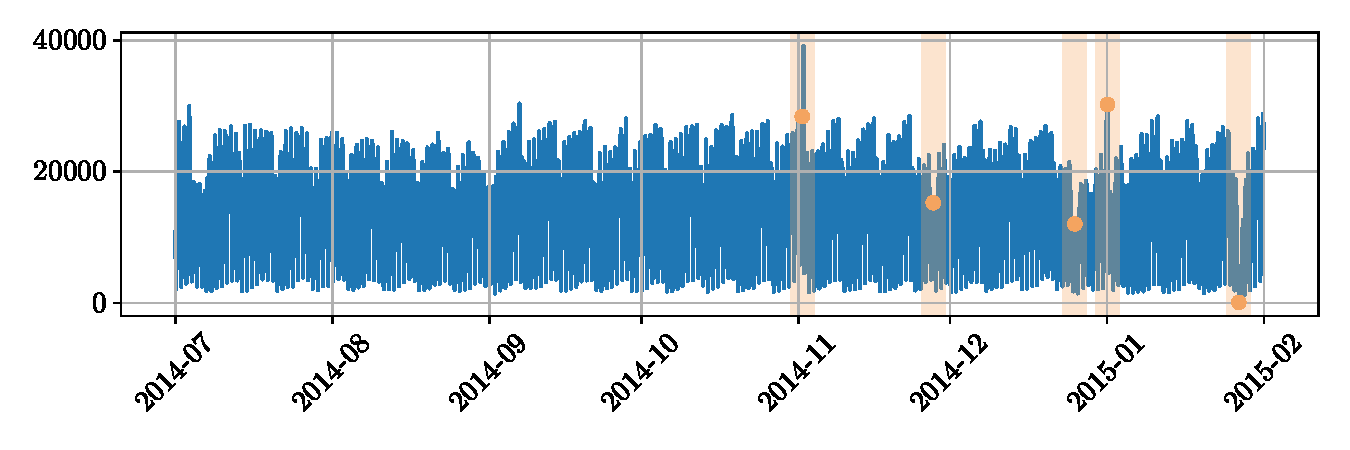
\includegraphics[width=0.7\linewidth]{./img/_ad_taxi_data.pdf}
    \caption{Plot of the time series, anomalies, and windows}
\end{figure}



\section{Approaches}


\subsection{Gaussian assumption}

Assuming that the data follows a Gaussian distribution, mean and variance can be used to determine anomalies through a threshold. $z$-score can also be used.


\subsection{Characterize data distribution}

Classify a data point as an anomaly if it is too unlikely.

\begin{description}
    \item[Formalization] 
        Given a random variable $X$ with values $x$ to represent the number of taxi calls, we want to find its probability density function (PDF) $f(x)$.

        An anomaly is determined whether:
        \[ f(x) \leq \varepsilon \]
        where $\varepsilon$ is a threshold.

        \begin{remark}
            The PDF can be reasonably used even though the dataset is discrete if its data points are sufficiently fine-grained.
        \end{remark}
\end{description}